% Input below the existing Generic CubeSat Structure section heading.
% The 18-paper count includes four RAX/enterprise predecessors and fourteen
% CRM/CSRM development or companion-method papers. It excludes application
% studies, specifications, and separately cited Space Symposium venue versions.
\label{section:generic-cubesat-structure}

The CubeSat System Reference Model (CSRM) is a reusable SysML model of a CubeSat mission's logical space and ground architecture. It links stakeholders, requirements, behaviors, technical measures and architecture to support the development of mission-specific models \citep{kaslow2020csrm}. The surveyed literature identifies 18 papers in its core research lineage, covering the Radio Aurora Explorer predecessors, reference model development, and companion methods for behavior, technical measurement, validation and mission engineering \citep{review-1646,review-1621,review-1554,review-1563,review-1494,review-1487,review-1451,review-1446,kaslow2017status3,kaslow2017behaviors,kaslow2018verification,review-1288,kaslow2018status4,kaslow2019csrm,kaslow2020csrm,review-1051,kaslow2022mission,rudder2026metamodel}. The International Council on Systems Engineering (INCOSE) Space Systems Working Group began investigating CubeSat modeling in 2011. Work progressed from mission demonstrations to a generic reference model and its validation, then to Object Management Group (OMG) specifications: CSRM 1.0 in 2023 and CSRM 1.1 in 2025 \citep{review-1494,kaslow2019csrm,omg2023csrm,omg2025csrm}. Applications include student CubeSat design through the Parkinson Sat 1U (PSAT1U) template, EPS conceptual design and concurrent engineering tutorials \citep{review-1112,review-1009,deutsch2022comet}. Its applicability to cislunar missions has also been assessed \citep{review-0699}.

The framework will use this reference structure as the starting point for its SysML v2 CubeSat model. Figures~\ref{fig:csrm-mission-structure}--\ref{fig:csrm-eps-components} show the mission structure, the nine CubeSat subsystems and the six EPS component groups. Mission teams will tailor these logical categories to their missions. Reference part multiplicities describe the template. Detailed design will establish physical quantities, electrical connections and implementation choices.
The CSRM EPS model will be tailored to each mission by selecting a topology alternative using the variation points defined by El Hachimi et al. \citep[Fig.~1, Sec.~4]{handpicked-0003}. Figure~\ref{fig:csrm-eps-topology} maps the relevant CSRM component groups to those choices.

% These authored views use the translated architecture from the 18 November
% 2025 CSRM model. The complete profile, behaviors and traceability are outside
% the current translation. The diagrams establish no SysML v2 conformance or
% runtime validation. The orbit reference is a chosen translation feature.

\begin{landscape}
\captionsetup{font=small,skip=4pt}
\begin{figure}[p]
\centering
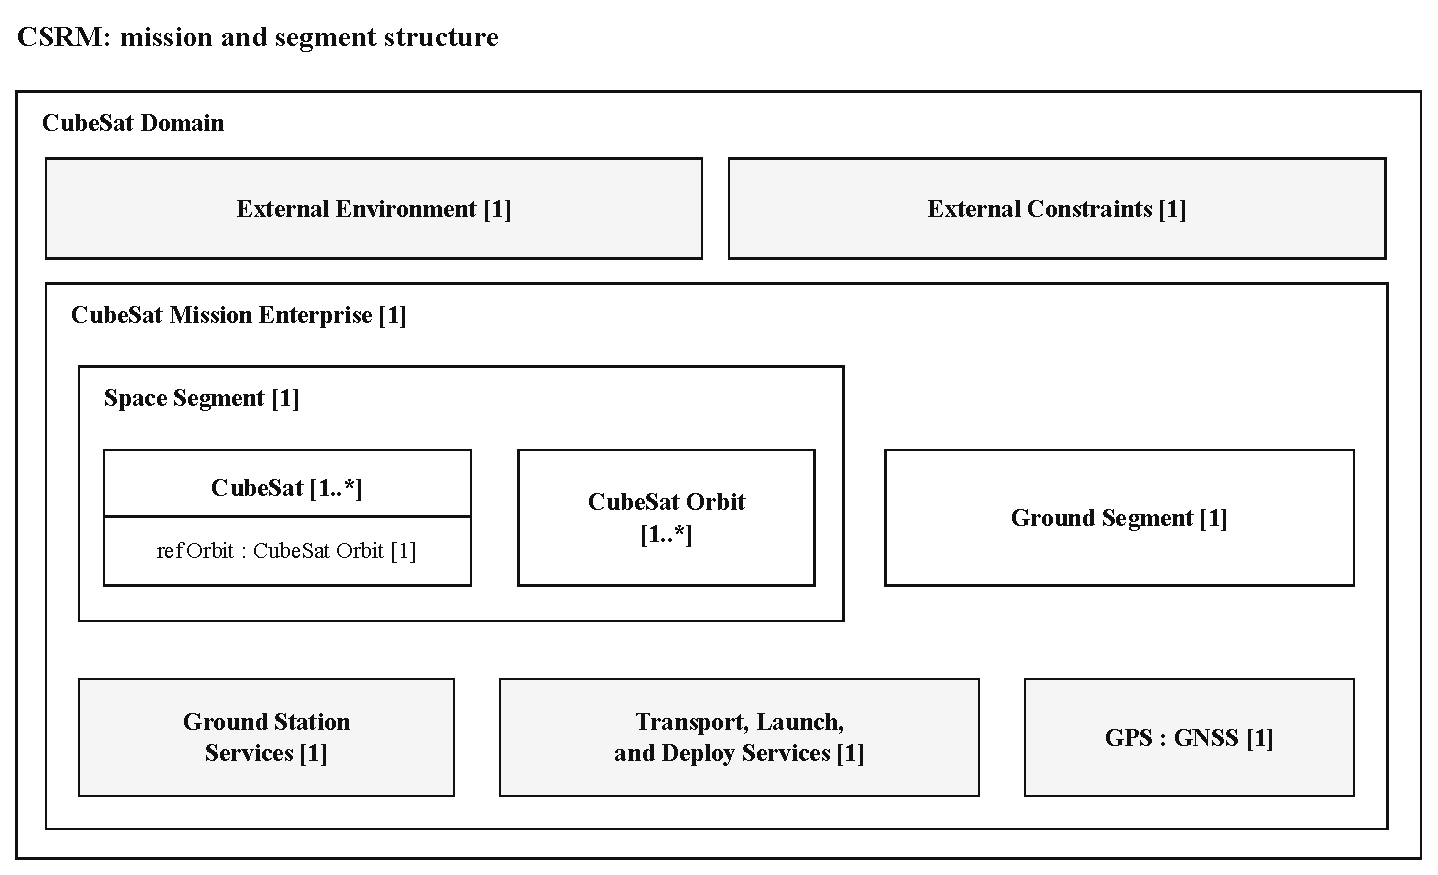
\includegraphics[width=\linewidth,height=\dimexpr\textheight-95pt\relax,keepaspectratio]{fig/csrm-mission-structure.pdf}
\caption[CSRM mission and segment structure.]{CSRM mission and segment structure. Nested rectangles denote composition. Brackets give part multiplicities. Light gray identifies external context and services. Orbits are modeled elements of the Space Segment. Each CubeSat has an orbit reference, with no individual spacecraft-to-orbit pairing specified in this view. Adapted from the CSRM reference model, copyright 2022 INCOSE Space Systems Working Group and OMG Space Domain Task Force, \href{https://creativecommons.org/licenses/by/4.0/}{CC BY 4.0} \citep{incose2025csrmmodel}.}
\label{fig:csrm-mission-structure}
\end{figure}
\clearpage

\begin{figure}[p]
\centering
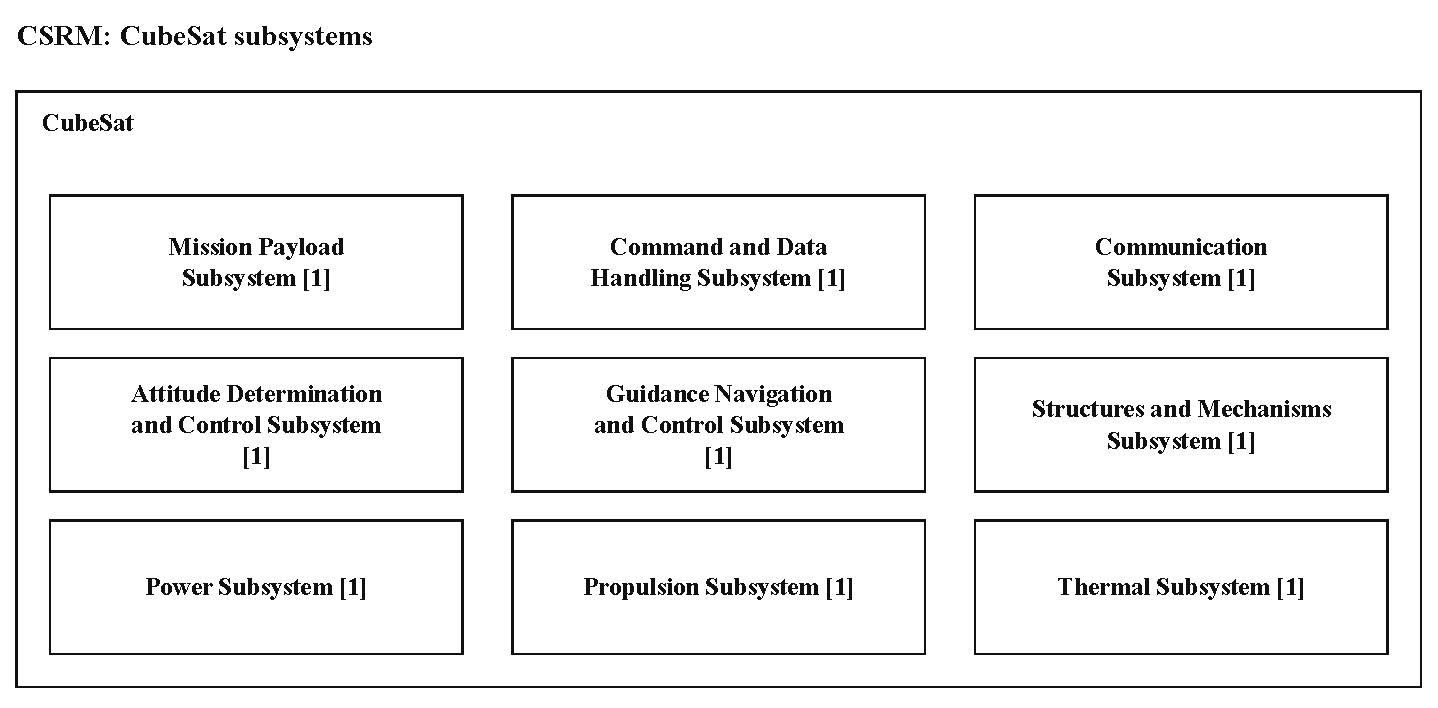
\includegraphics[width=\linewidth,height=\dimexpr\textheight-80pt\relax,keepaspectratio]{fig/csrm-cubesat-subsystems.pdf}
\caption[CSRM CubeSat subsystems.]{CSRM CubeSat subsystems. The reference architecture contains one part for each of nine subsystem categories. Power Subsystem is the EPS. Mission-specific models can omit, combine or refine categories to meet mission needs \citep{kaslow2020csrm}. The view shows logical composition. It specifies no subsystem interfaces or allocation to circuit boards. Adapted from the CSRM reference model \citep{incose2025csrmmodel}.}
\label{fig:csrm-cubesat-subsystems}
\end{figure}
\clearpage

\begin{figure}[p]
\centering
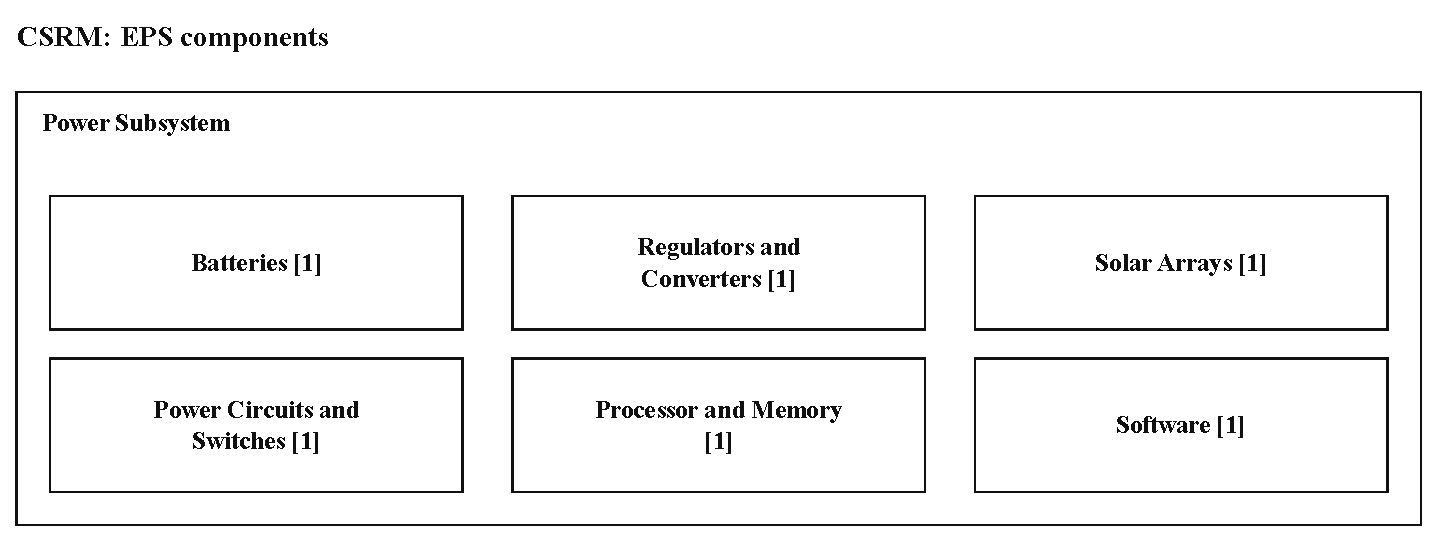
\includegraphics[width=\linewidth,height=\dimexpr\textheight-80pt\relax,keepaspectratio]{fig/csrm-eps-components.pdf}
\caption[CSRM EPS component groups.]{CSRM EPS component groups. The Power Subsystem contains six reference component categories, including processing and software. Batteries and Solar Arrays each denote an aggregate category. Multiplicity [1] identifies one reference part per category. Detailed design will define the numbers of cells, panels, converters and switches, together with their electrical connections. Adapted from the CSRM reference model \citep{incose2025csrmmodel}.}
\label{fig:csrm-eps-components}
\end{figure}
\clearpage
\begin{figure}[p]
\centering
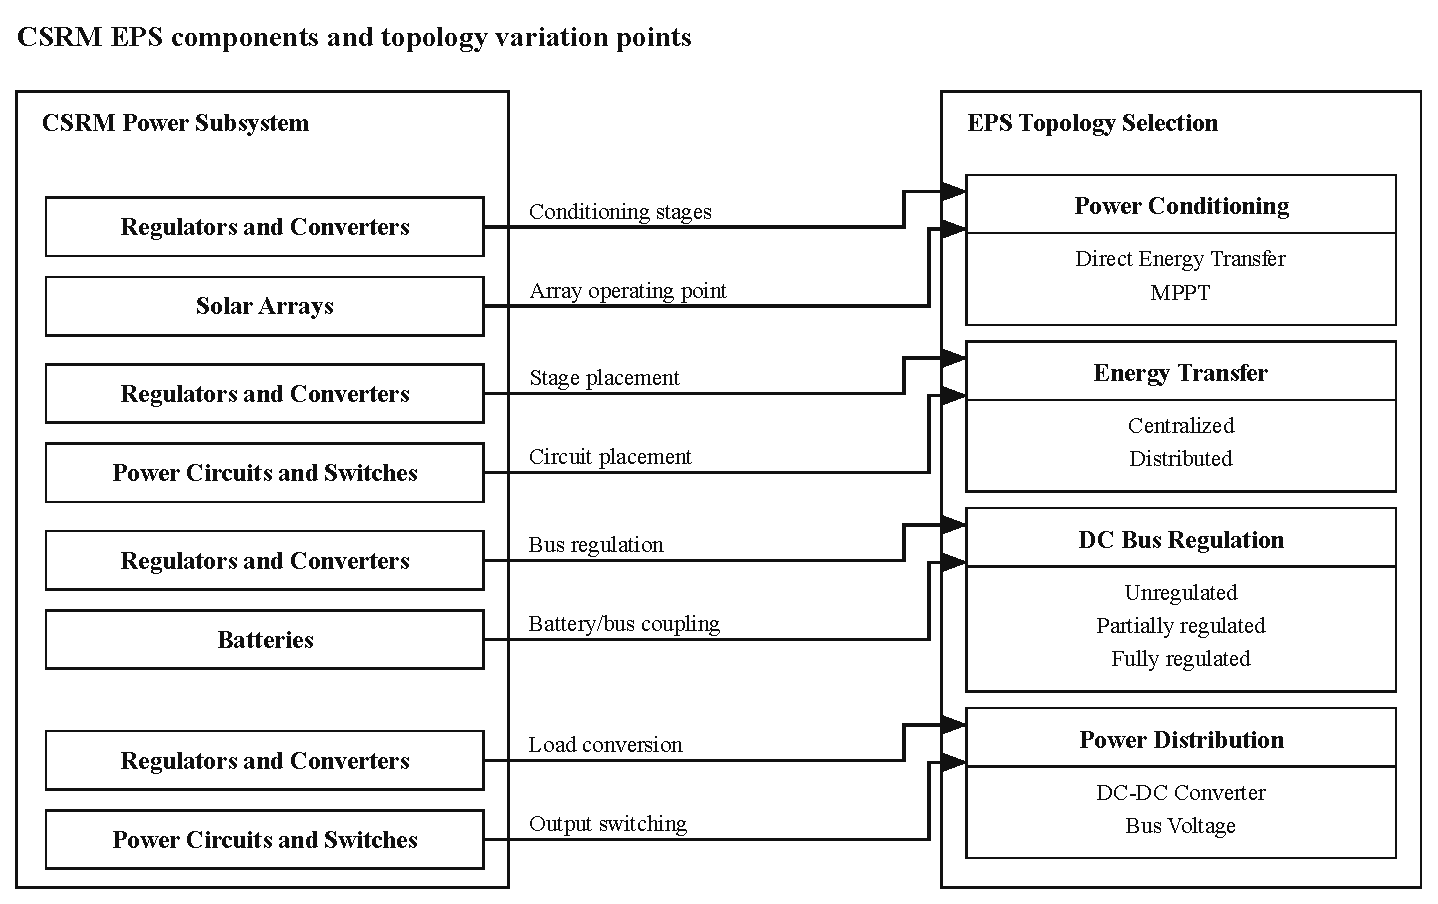
\includegraphics[width=\linewidth,height=\dimexpr\textheight-95pt\relax,keepaspectratio]{fig/csrm-eps-topology.pdf}
\caption[CSRM EPS components and topology variation points.]{CSRM EPS components and topology variation points. Arrows express design associations proposed for this framework. Route labels identify the affected design roles. Repeated component names denote the same CSRM groups \citep{incose2025csrmmodel}. The alternatives follow El Hachimi et al. \citep[Fig.~1, Sec.~4]{handpicked-0003}. The view focuses on hardware topology. Processing and software remain in the reference structure shown in Figure~\ref{fig:csrm-eps-components}. No topology alternative is selected in this view.}
\label{fig:csrm-eps-topology}
\end{figure}
\clearpage
\end{landscape}
